\chapter{Pengelolahan File CSV}
\section{Pemahaman Teori}
\begin{enumerate}
    \item Apa itu fungsi file csv, jelaskan sejarah dan contoh
    \begin{itemize}
        \item 
        \textbf{Pengenalan CSV} \\
        \hspace*{1cm} Comma Separated Values (CSV) sebuah text yang bisa berisi daftar data-data. CSV adalah suatu format data yang di mana setiap bagian data dipisahkan dengan tanda koma (,) atau dengan tanda titik koma (;). Format CSV biasanya berfungsi untuk menukar atau mengonversi data ke format lainnya. CSV mempermudah untuk mengimport kan sebuah data kedalam aplikasi. 
        \item 
        \textbf{Sejarah format CSV} \\
        \hspace*{1cm}Pada tahun 1972 IBM Fortran (level H extended) compiler dibawah  OS / 360 sudah mendukung format CSV. Pada saat itu Fotran 77 mendefinisikan penulisannya pada input/output ditulis menggunakan tanda koma atau spasi untuk membatasi antar datanya akhirnya disetujui pada tahun 1978. Input yang diarahkan daftar menggunakan koma atau spasi untuk pembatas, sehingga string karakter yang tidak dikutip tidak dapat mengandung koma atau spasi.
        
        \hspace*{1cm}Nama "nilai yang dipisahkan koma" dan singkatan "CSV" digunakan pada tahun 1983. Manual untuk komputer Osborne Executive, yang menggabungkan SuperCalc spreadsheet, mendokumentasikan konvensi kutipan CSV yang memungkinkan string berisi koma yang disematkan, tetapi manual tersebut tidak menentukan konvensi untuk menyematkan tanda kutip dalam string yang dikutip. Daftar nilai yang dipisahkan koma lebih mudah untuk diketik (misalnya ke dalam kartu berlubang) daripada data yang selaras dengan kolom tetap dan cenderung menghasilkan hasil yang salah jika suatu nilai dilubangi satu kolom dari lokasi yang dituju.. 
        
        \hspace*{1cm}Pada Tahun 2005 inisiatif standardisasi utama - mentransformasikan "definisi fuzzy de facto" menjadi definisi yang lebih tepat dan de jure. dengan RFC4180, mendefinisikan CSV sebagai Tipe Konten MIME. Kemudian, pada 2013, beberapa kekurangan RFC4180 ditangani oleh rekomendasi W3C.
        
        \hspace*{1cm}IETF menerbitkan RFC7111 yang menjelaskan aplikasi fragmen URI pada dokumen CSV  pada tahun 2014 . RFC7111 menentukan bagaimana penggunaan rentang baris, kolom, dan sel dapat dipilih dari dokumen CSV menggunakan indeks posisi.
       
        \hspace*{1cm}W3C, dalam upaya untuk meningkatkan CSV dengan semantik formal, mempublikasikan draft rekomendasi pertama untuk standar metadata CSV, yang dimulai sebagai rekomendasi pada bulan Desember tahun yang sama Pada 2015.
       
	\item Contoh Penggunaan Format CSV
	\lstinputlisting[firstline=1, lastline=4]{src/teori1.csv}
	\end{itemize}
	
    \item Aplikasi-aplikasi apa saja yang bisa menciptakan file csv?
	\begin{enumerate}
		\item Editor teks (Notepad, Sublime, VS Code, Atom, dan lain-lain)
		\item Spreadsheet (Microsoft Excel, google spreadshare, LibreOffice dan lain-lain)
	\end{enumerate}
		
	\item Jelaskan bagaimana cara menulis dan membaca file csv di excel atau spreadsheet	
	\textbf{Menulis File CSV}
	\begin{enumerate}
		\item Pertama silahkan buka aplikasi Excel dengan cara klik ''Start'', cari Excel, kemudian tekan Enter.
		
	
		\item Setelah aplikasi terbuka silahkan klik ''Blank Workbook''.
		
		\begin{figure}[!htbp]
			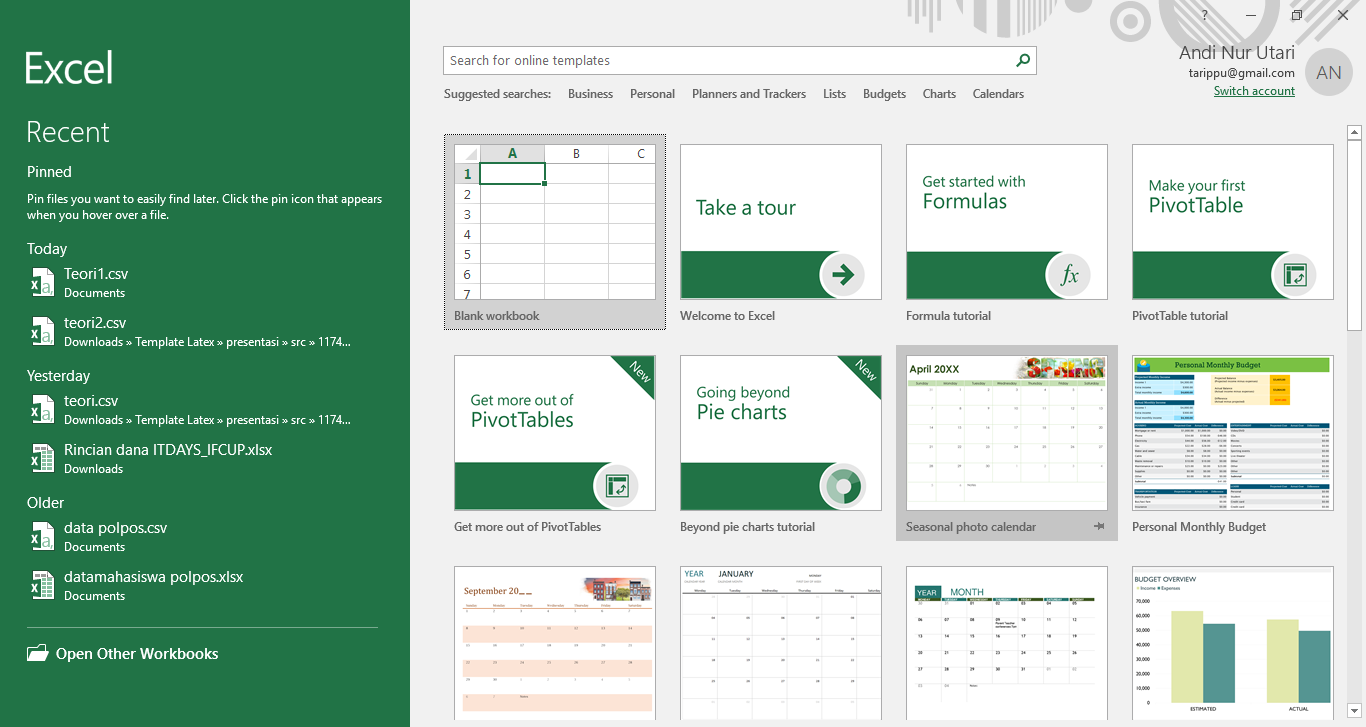
\includegraphics[width=10cm]{figures/a1.PNG}
			\centering
		\end{figure}
		\newpage
		
		\item Kemudian isi sesuai dengan data yang ingin dibuat.
		
		\begin{figure}[!htbp]
			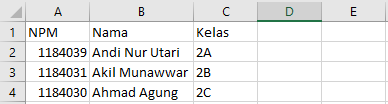
\includegraphics[width=10cm]{figures/a2.PNG}
			\centering
		\end{figure}
		
		\item Setelah selesai dibuat, silahkan simpan file tersebut dengan cara mengklik ''File'', lalu klik ''Save''.
		
		\begin{figure}[!htbp]
			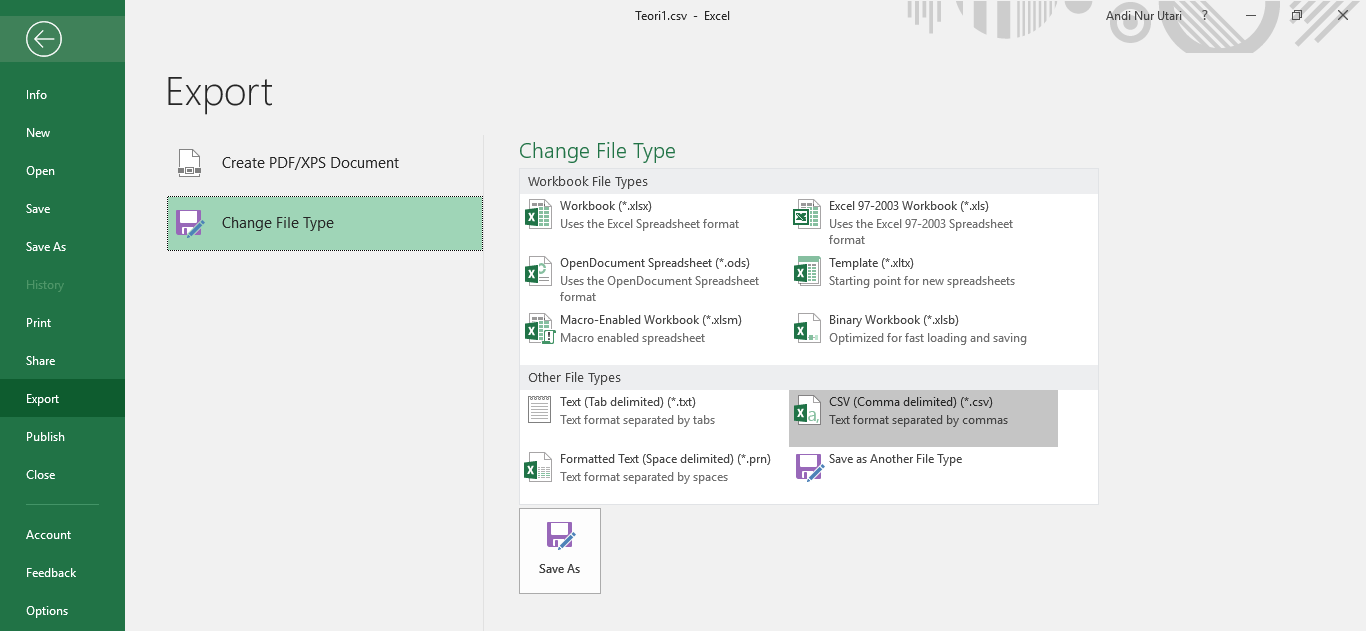
\includegraphics[width=10cm]{figures/a3.PNG}
			\centering
		\end{figure}
		\newpage
		
		\item Kemudian isi kolom ''File name'' dengan nama file anda dan kolom ''Save as type'' pilih yang berekstensi .csv.
		
		\begin{figure}[!htbp]
			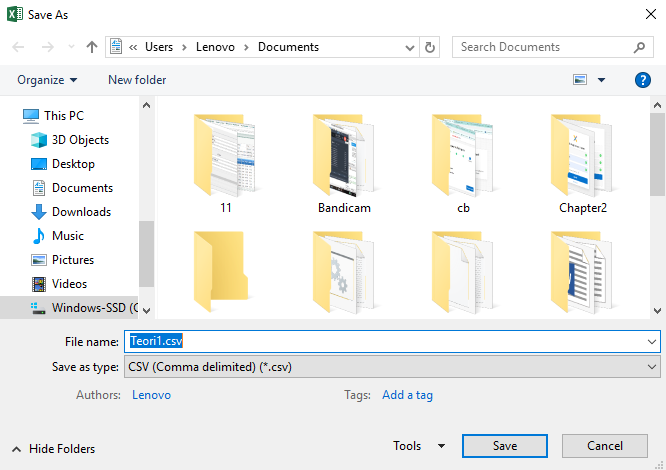
\includegraphics[width=9cm]{figures/a4.PNG}
			\centering
		\end{figure}
		
		\item Lalu tinggal klik ''Yes''.
			\begin{figure}[!htbp]
			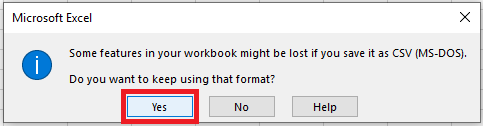
\includegraphics[width=9cm]{figures/t6.png}
			\centering
		\end{figure}
		
		\item Kemudian file yang Anda telah terbuat tadi tersimpan dengan ekstensi .csv. Untuk melihat isi filenya tinggal klik dua kali pada file tersebut.
		
		\begin{figure}[!htbp]
			
\includegraphics[width=2cm]{figures/a5.png}
			\centering
		\end{figure}
		
		\item Berikut ini adalah isi dari file yang tadi Anda buat.
		
		\begin{figure}[!htbp]
			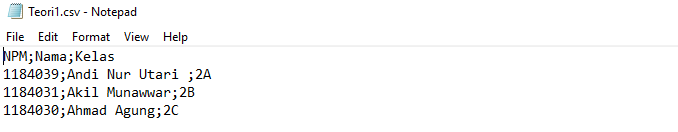
\includegraphics[width=12cm]{figures/a6.PNG}
			\centering
		\end{figure}
	\end{enumerate}
	
	\newpage
	\textbf{Melihat File CSV di Excel atau Spreadsheet}
	
	\begin{enumerate}
		\item Pertama klik dua kali pada file yang yang berekstensi CSV.
		
		\begin{figure}[!htbp]
			
\includegraphics[width=2cm]{figures/a5.PNG}
			\centering
		\end{figure}
		
		\item Kemudian file akan terbuka secara otomatis di aplikasi Excel atau spreadsheet.
		
		\begin{figure}[!htbp]
			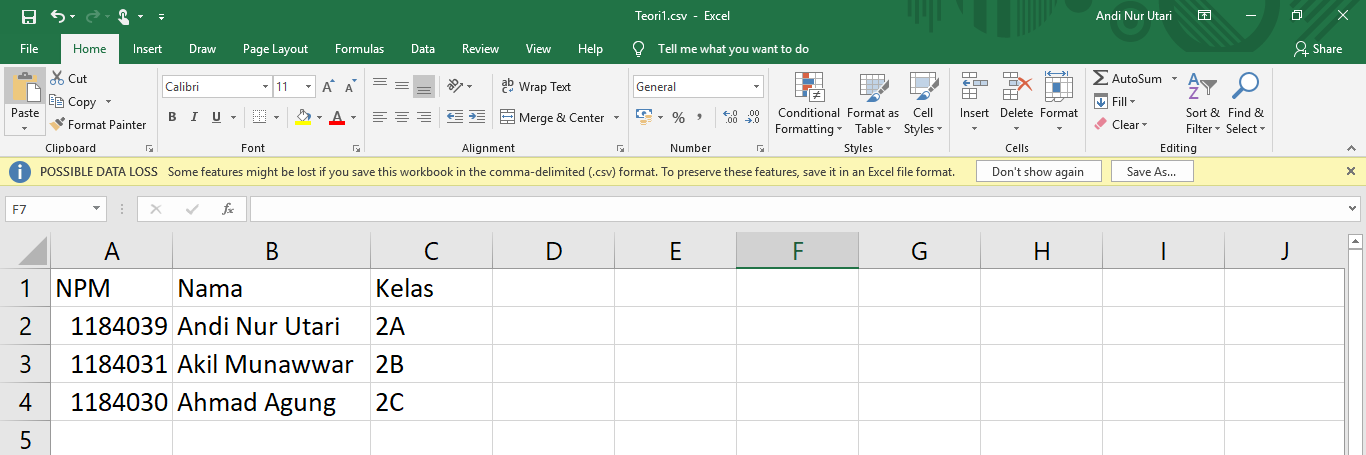
\includegraphics[width=10cm]{figures/a8.PNG}
			\centering
		\end{figure}
	\end{enumerate}
	
	\item Sejarah library csv
	
	\hspace*{1cm}Library csv mengimplementasikan kelas untuk membaca dan menulis data tabular dalam format CSV. Hal ini memungkinkan programmer untuk mengatakan, "tulis data ini dalam format yang disukai oleh Excel," atau "baca data dari file ini yang dihasilkan oleh Excel," tanpa mengetahui detail yang tepat dari format CSV yang digunakan oleh Excel. Pemrogram juga dapat menggambarkan format CSV yang dipahami oleh aplikasi lain atau menentukan format CSV tujuan khusus mereka sendiri.
	
	\newpage 
	\item Sejarah library pandas
	
	\hspace*{1cm}Pada 2008, pengembangan pandas dimulai di AQR Capital Management. Pada akhir 2009 telah menjadi open source, dan secara aktif didukung hari ini oleh komunitas individu yang berpikiran sama di seluruh dunia yang menyumbangkan waktu dan energi berharga mereka untuk membantu membuat panda open source menjadi mungkin.
	
	\hspace*{1cm}Sejak 2015, pandas adalah proyek yang disponsori NumFOCUS. Ini akan membantu memastikan keberhasilan pengembangan panda sebagai proyek sumber terbuka kelas dunia.
	
    \item Fungsi-fungsi yang terdapat di library csv, yaitu:
	\begin{enumerate}
		\item Reader
		 Fungsi ini digunakan untuk membaca isi file berformat CSV dari list.
		
		\lstinputlisting[language=Python, firstline=10, lastline=15]{src/csv.py}
		
		\item DictReader
		
		Fungsi ini digunakan untuk membaca isi file berformat CSV dari dictionary.
		
		\lstinputlisting[language=Python, firstline=18, lastline=23]{src/csv.py}
		
		\item write
		
		Fungsi ini digunakan untuk menulis file berformat CSV dari list.
		
		\lstinputlisting[language=Python, firstline=27, lastline=33]{src/csv.py}
		
		\item DictWrite
		
		Fungsi ini digunakan untuk menulis file berformat CSV dari dictionary.
		
		\lstinputlisting[language=Python, firstline=37, lastline=46]{src/csv.py}
		
	\end{enumerate}
	
	\item Fungsi-fungsi yang terdapat di library pandas, yaitu:
	\begin{enumerate}
		\item read\_csv
		
		Fungsi ini digunakan untuk membaca isi file berformat CSV
		
		\lstinputlisting[firstline=9, lastline=12]{src/pandasnw.py}
		
		\item to\_csv
		
		Fungsi ini digunakan untuk menulis file berformat CSV
		
		\lstinputlisting[firstline=15, lastline=18]{src/pandasnw.py}
		
	\end{enumerate}
\end{enumerate}


\newpage
\section{Keterampilan Pemrograman}
\begin{enumerate}
	\item Buatlah  fungsi  (file  terpisah/library  dengan  nama  NPMcsv.py)  untuk  membuka file csv dengan lib csv mode list.
	\lstinputlisting[firstline=10, lastline=15]{src/1184039csv.py}
	
	\item Buatlah  fungsi  (file  terpisah/library  dengan  nama  NPMcsv.py)  untuk  membuka file csv dengan lib csv mode dictionary.
	\lstinputlisting[ firstline=17, lastline=22]{src/1184039csv.py}
	
	\item Buatlah fungsi (file terpisah/library dengan nama NPMpandas.py) untuk membuka file csv dengan lib pandas mode list.
	\lstinputlisting[ firstline=10, lastline=13]{src/1184039pandas.py}
	
	\item Buatlah fungsi (file terpisah/library dengan nama NPMpandas.py) untuk membuka file csv dengan lib pandas mode dictionary.
	\lstinputlisting[firstline=10, lastline=13]{src/1184039pandas.py}
	
	\item  Buat fungsi baru di NPMpandas.py untuk mengubah format tanggal menjadi standar dataframe.
	\lstinputlisting[firstline=15, lastline=19]{src/1184039pandas.py}
	
	\item Buat fungsi baru di NPMpandas.py untuk mengubah index kolom.
	\lstinputlisting[firstline=21, lastline=24]{src/1184039pandas.py}
	
	\item Buat fungsi baru di NPMpandas.py untuk mengubah atribut atau nama kolom.
	\lstinputlisting[firstline=26, lastline=30]{src/1184039pandas.py}
	
	\item Buat program main.py yang menggunakan library NPMcsv.py yang membuat dan membaca file csv.
	\lstinputlisting[firstline=8, lastline=13]{src/main.py}
	
	\item Buat program main2.py yang menggunakan library NPMpandas.py yang membuat dan membaca file csv.
	\lstinputlisting[firstline=8, lastline=13]{src/main2.py}
	
\end{enumerate}
\newpage
\section{Keterampilan Penanganan Eror}
\begin{enumerate}
	\item Tuliskan  peringatan  error  yang  didapat  dari  mengerjakan  praktek  keempat  ini, dan  jelaskan  cara  penanganan  error  tersebut.   dan  Buatlah  satu  fungsi  yang menggunakan gunakan try except untuk menanggulangi error tersebut.
	
	Peringatan error di praktek keempat ini, yaitu:
	\begin{itemize}
		\item Syntax Errors
		Syntax error adalah suatu keadaan atau kondisi ketika ada kesalahan penulisan kode pada program python hal ini menyebabkan program tidak dapat dijalankan. contohnya kesalahan pemberian titik dua atau tanda kutip. Output pemberitahuan error nya yaitu invalid syntax. Yang harus dilakukan saat terjadi syntax error pada kode program yaitu memperbaiki penulisan kodenya.
		
		\item Name Error
		NameError adalah exception yang terjadi saat kode melakukan eksekusi terhadap local name atau global name yang tidak terdefinisi. Cara mengatasi name error adalah memastikan variabel atau function yang dipanggil ada atau tidak salah ketik.
		
		\item Type Error
		TypeError adalah exception yang akan terjadi apabila pada saat dilakukannya eksekusi terhadap suatu operasi atau fungsi dengan type object yang tidak sesuai. cara mengatasi dari error ini adalah mengkoversi varibelnya sesuai dengan tipe data yang akan digunakan.
		
		\item Identation error
        Identation error, yaitu tulisasn kode program yang menjorok. identation error akan terjadi ketika mengetik kode program namun tidak memperhatikan identasinya. Jika terjadi identasi maka program akan error. cara mengatasinya yaitu memperhatikan identasi saat menuliskan suatu program.
\end{itemize}
\newpage
	\item Penggunaan Try except
	\lstinputlisting[firstline=8, lastline=22]{src/try.py}
\end{enumerate}

\textbf{Cek Plagiat}
\begin{figure}[!htbp]
	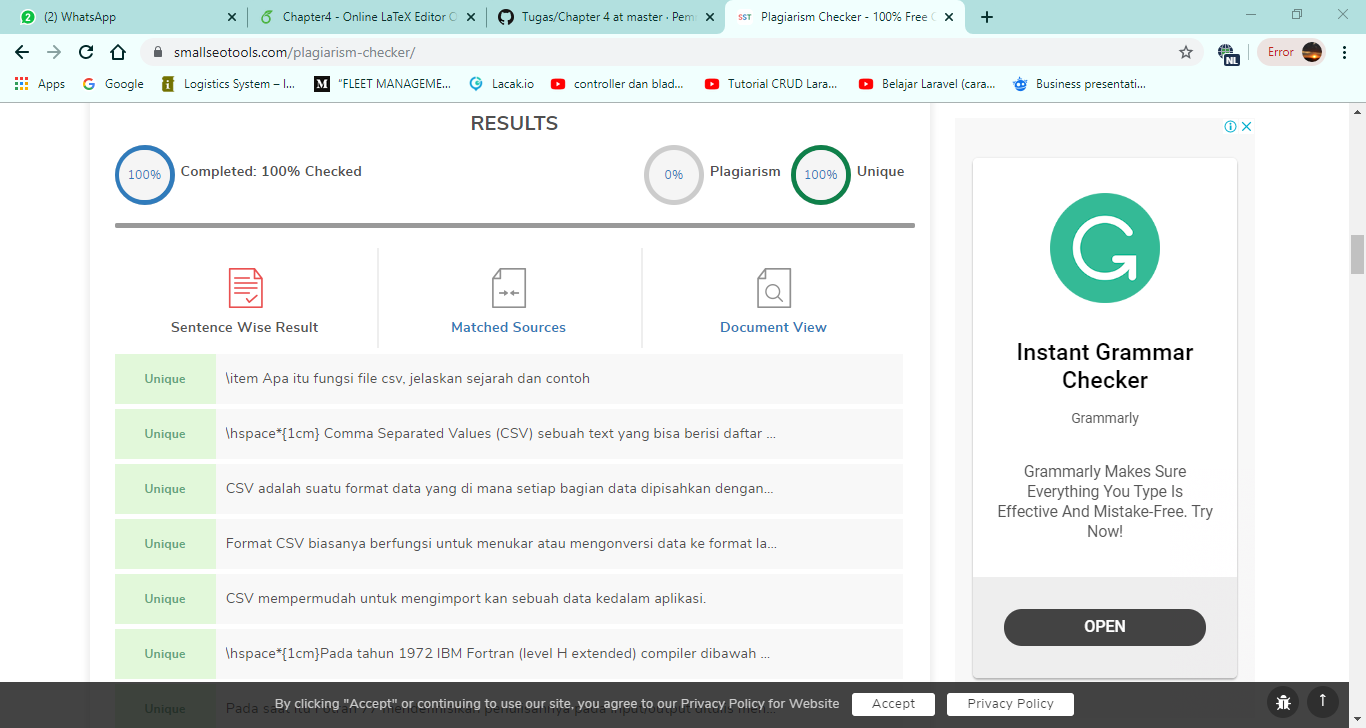
\includegraphics[width=10cm]{figures/plagiat1.PNG}
	\centering
\end{figure}
\begin{figure}[!htbp]
	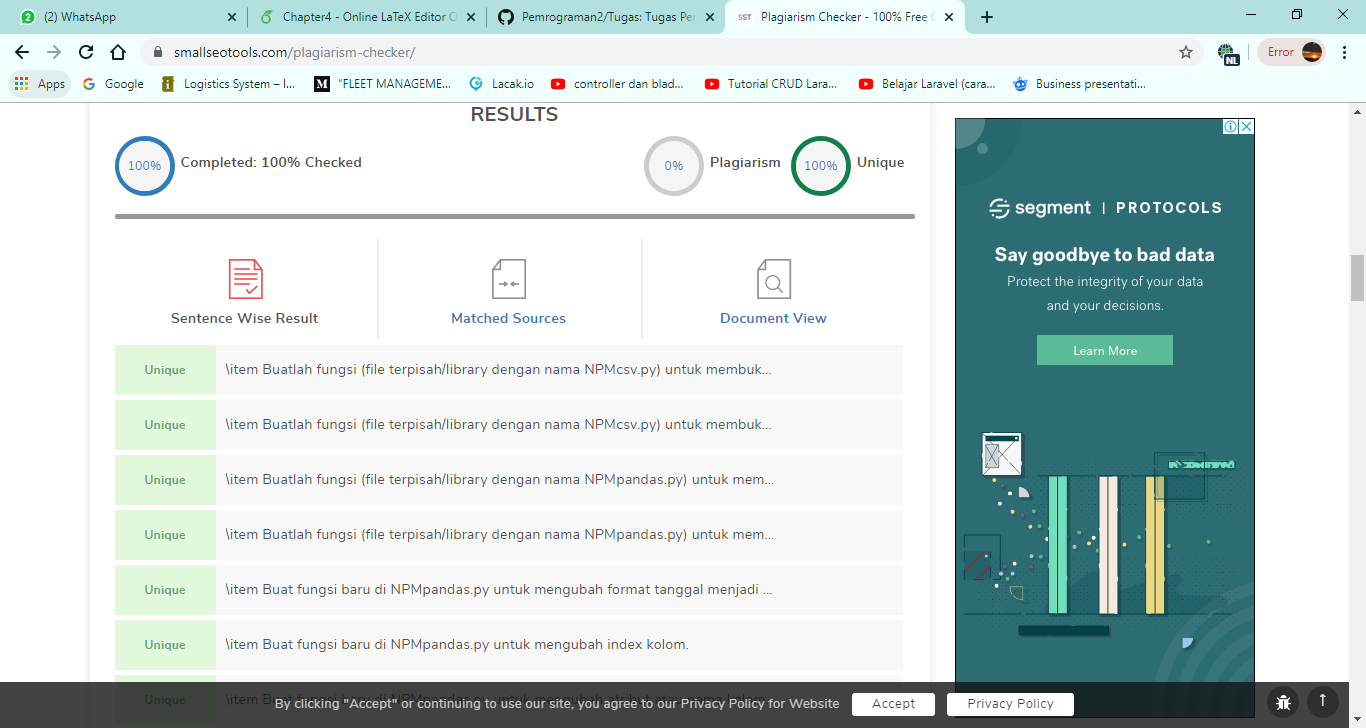
\includegraphics[width=10cm]{figures/plagiat2.PNG}
	\centering
\end{figure}
	
	

    
    
